\documentclass[12pt]{article}
\usepackage[a4paper, margin=2cm]{geometry}
\usepackage[english]{babel} % To obtain English text with the blindtext package
\usepackage{blindtext}
\usepackage{graphicx} % Required for inserting images
\usepackage{array} % For extra column formatting
\usepackage{amsmath} %for equation environment
\usepackage{float}
\usepackage{parskip} % For gaps between para
\usepackage{setspace}
\usepackage{pdfpages}
\usepackage{abstract}
\usepackage[export]{adjustbox}
\usepackage{emptypage}
\usepackage{tocloft}
\usepackage[nottoc]{tocbibind}
\usepackage{hyperref, url}
\usepackage{subcaption}
\usepackage{lipsum}
\usepackage{xcolor}
\usepackage{caption}
    \captionsetup{font=footnotesize,labelfont=bf}

\cftsetindents{section}{0em}{2em}
\cftsetindents{subsection}{0em}{2em}

\renewcommand\cfttoctitlefont{\hfill\Large\bfseries}
\renewcommand\cftaftertoctitle{\hfill\mbox{}}

\graphicspath{ {./images/} }

\pagenumbering{arabic}

\definecolor{blurple}{HTML}{5865F2}

\hypersetup{
    colorlinks=true,
    linkcolor=black,
    urlcolor=blurple,
    citecolor=blurple,
}

\urlstyle{same}
%%%%%%%%%%%%%%%%%%%%%%%%%%%%%%%%%%%


\title{PHYC20090 Exp.7 LCR Circuits}
\author{Joana Adao}
\date{\today}

\begin{document}

\begin{titlepage}
    \begin{center}

        \begin{figure}[ht]
            
\includegraphics[width=\textwidth]{UCDLogo.png}
        \end{figure}
        
        \begin{figure}
            \centerline{
\includegraphics[width=\paperwidth]{UCDBanner.png}}
        \end{figure}

        \vspace{4cm}

        {\Huge \bfseries PHYC20090 Electronics and Devices}\\
        \vspace{0.75cm}
        {\LARGE Experiment No.7 Sinusodial Response of the LCR Resonant Circuit }
        
        \vspace{1cm}
    
    {\Large \textbf{27 January 2025 }}

    \vspace{2cm}
    
    {\large \textbf{by Joana C.C. Adao (Student No. 23311051)}}\\
    \medskip
    {\large With Arminas A., Ananya L., Samuel S.}

    \end{center}
    
   \clearpage

\end{titlepage}

\setcounter{page}{1}
\tableofcontents

\newpage

\begin{abstract}
\addcontentsline{toc}{section}{Abstract}

The aim of this experiment was to



\end{abstract}


%%%%%%%%%%%%%%%%%%%%%%%%%%%%%%%%%%%


\section{Theory}

\subsection{LCR Circuits} \label{sec:1.1}
An LCR circuit is made up of inductors (L), capacitors (C), and resistors (R), usually connected in series.
Since all the components of the circuit are connected in series, equal amount of the current will flow through each element.
\cite{unacademy}

A circuit containing these components, L, C, and R, can act as themselves individually at certain frequencies
\cite{learnabout}.
The LCR circuit can also magnify the voltages across the L, C, and R such that it is larger than the  circuit's input voltage (ie. AC, Alternating Current)
\cite{learnabout}.

\subsubsection{Inductance, Capacitance, Resistance} \label{sec:1.1.1}

Inductance, capacitance, and resistance make up the basic parameters that can affect circuits up to some degree
\cite{elecnotes}.

\textbf{Inductance} is a property of a conductor
\cite{britinductance}
and it's measured by its ability to store energy due to the magnetic field produced by the flow of current
\cite{elecnotes}
and the voltage that is induced by the current's rate of change
\cite{britinductance}.
With AC (Alternating Current), the magnetic field produced fluctuates with the time-varying properties of AC power sources
\cite{elecnotes,britinductance}.

The voltage is proportional to the rate of change of the current and this factor of proportionality is known as the inductance
\cite{britinductance}.
Coils of wire are most commonly used as the inductors in circuits as they amplify \cite{elecnotes} the efficiency at which the magnetic field induces
the voltage and current in the circuit. By coiling wire (solenoid) the magnetic field is concentrated and magnified at its centre, shown in Figure \ref{fig:solenoid}.

\begin{figure}[H]
    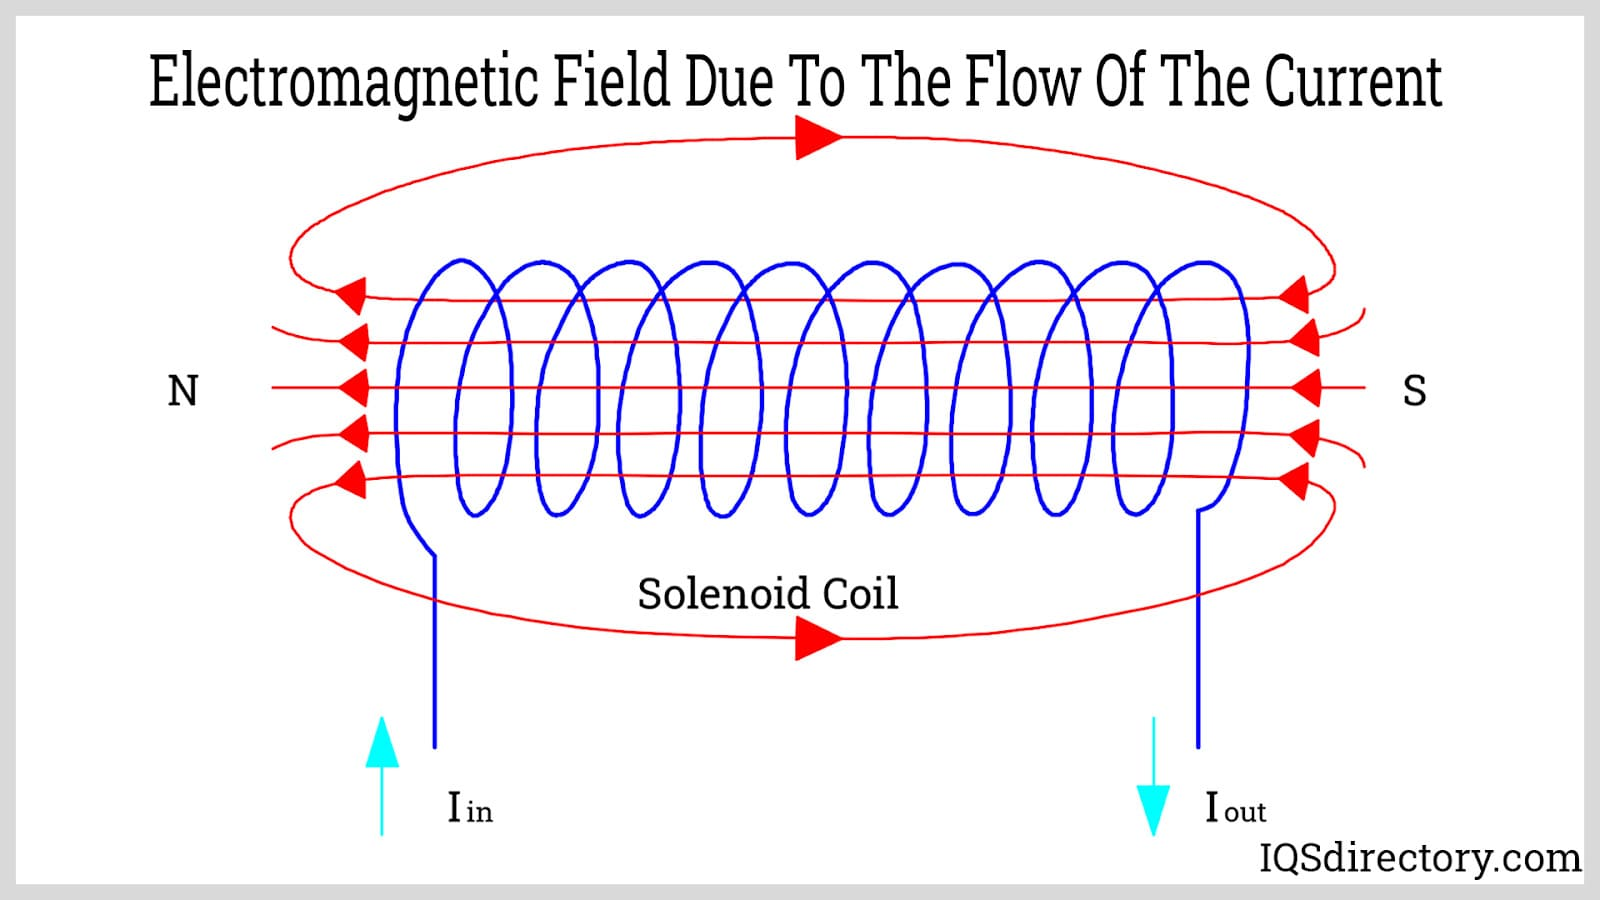
\includegraphics[width=15cm]{solenoid.jpg}
    \centering
    \caption{\centering \footnotesize{Electromagnetic Field Due to the Flow of the Current in a Solenoid \cite{solenoidpic}}}
    \label{fig:solenoid}
\end{figure}

\textbf{Capacitance} is a circuit's, or circuit component's, ability to collect and store electric charge
\cite{flukecapacitance}.
Capacitors are made up of two electrically conductive plates separated by some distance. These two plates, when voltage is exchanged between them,
become equally charged such that one plate is negatively charged (-Q) and the other is positively charged (+Q)
\cite{britcapacitance,librecapacitance}.
Overall, the charge of the capacitor will be neutral as the equal charge from both plates (-Q, +Q) cancels out
\cite{librecapacitance} as in figure \ref{fig:ppcapacitor}.

In a circuit with an AC supply, the capacitor is alternatively charged and discahrged every half cycle, therefore the amount of total
stored charge in that capacitor depends on the frequency of the AC supply as it dictates how long it will charge for
\cite{britcapacitance}.

Capacitors are usually assembled with a dielectric material inbetween the two conductive plates
\cite{britcapacitance,flukecapacitance,librecapacitance}.
Dielectric materials are poor conductors of electric fields, therefore labelled as insulators 
\cite{britdielectric}.
The capacitance of a capacitor increases with a dielectric material as the electric field is decreased and in turn so is the voltage across the two plates
\cite{hyperdielectric}.
The capacitor ends up storing the same charge as if it were without a dielectric material but at a lower voltage, which is effective in reducing the possibilites of a circuit short
\cite{hyperdielectric}.

\begin{figure}[H]
    \centering
    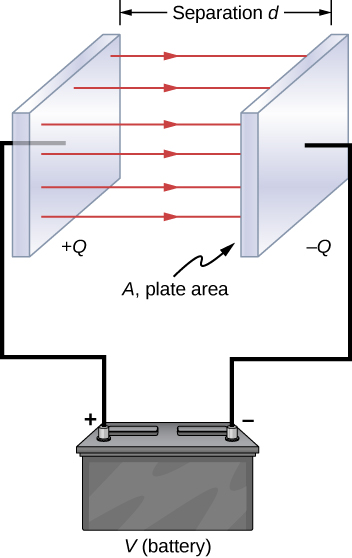
\includegraphics[width=5cm]{parallel plate capacitor.jpg}
    \caption{\centering \footnotesize{Parallel Plate Capacitor Diagram \protect\cite{librecapacitance}}}
    \label{fig:ppcapacitor}
\end{figure}

\textbf{Resistance} is a force that opposes the flow of current in a circuit
\cite{flukeresistance,hiokiresistance,britresistance}.
It can be described as the electrical charge's difficulty in moving through a material.
\cite{hiokiresistance}
Conductors and insulators, mentioned before, are types of materials classified by their resistance. Conductors are materials with little resistance that the
electrons can travel through easily, like copper and gold (most metals). Insulators, on the other hand, are materials that make it difficult for the electrical
charge to pass through, like wood and rubber
\cite{flukeresistance}.
These properties can be seen in electrical wires, with the current-carrying copper wire is encased in an insulating rubber tube for safety.

The resistance of a circuit component usually increases with temperature as the atoms that make up that material get excited, moving around in ways that make it
difficult for the electrons to travel through
\cite{britresistance,bbcresistance}.

Resistors are circuit components specifically made to counteract the flow of current in a circuit
\cite{britresistor,bbcresistance,hiokiresistance} (Figure).
Resistors can be used in a circuit to control the amount of voltage and current flowing in a circuit, which is useful to make sure the circuit doesn't blow and also
to correctly distribute the current/voltage throughout the circuit
\cite{britresistor,hiokiresistance}
The surplus of electrical energy flowing through a resistor is converted into heat energy which then dissipates
\cite{hiokiresistance}.

\begin{figure}[H]
    \centering
    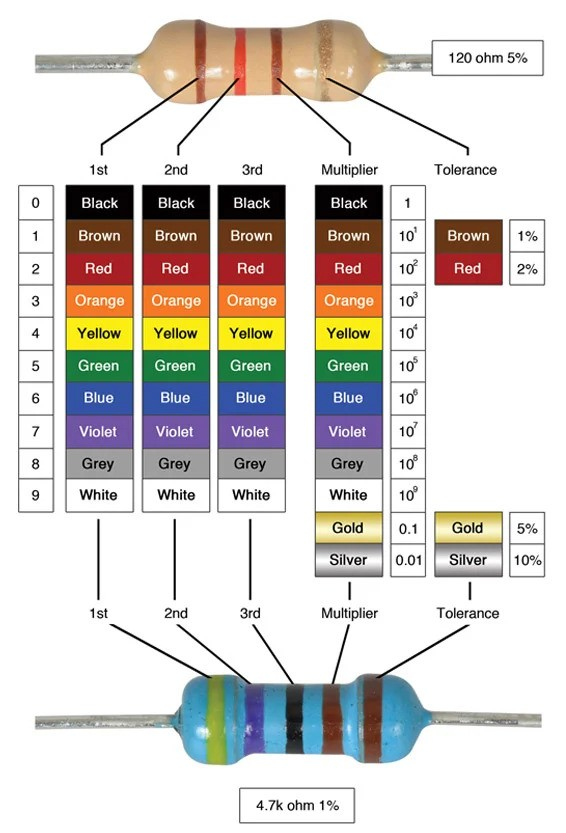
\includegraphics[width=7.5cm]{resistorr.jpg}
    \caption{\centering \footnotesize{Resistor and How to Read One \protect\cite{resistorpic}}}
    \label{fig:resistor}
\end{figure}

\subsubsection{Impedance} \label{sec:1.1.2}

The impedance of a circuit represents the overall resistance that it offers to AC
\cite{lionimpedance}.
The difference between resistance and impedance is that impedance only truly affects AC circuits while resistance affects both AC and DC (Direct Current)
\cite{isaacimpedance,protimpedance}.
In AC circuits the current is not constant but instead alternating, so the usual ratio of $\dfrac{V}{I}$ will also not be constant
\cite{isaacimpedance}.

Impedance is the vector sum of the resistance (R), when the current is in phase and peaks at the same time, and reactance (X), which peaks one quarter of the cycle,
within the circuit
\cite{lionimpedance,isaacimpedance}.
The reactance X is composed of the positive reactance of the inductor ($X_L$) and the negative reactance of the capacitor ($X_C$)
\cite{isaacimpedance}.

Impedance will be mathematically expanded on in §\ref{sec:1.3}, The Mathematics.

\subsection{Wave Properties} \label{sec:1.2}

Charged particles can create electromagnetic fields with their movement which transports
electromagnetic (EM) energy, like light and radiation.
They generate both an electric field and magnetic field, as the name implies
\cite{NASAemwave}.
Electromagnetic waves do need a material in order to be able to move, unlike mechanical waves
\cite{NASAemwave}.
As EM waves propagate, the frequency at which they're moving at has its own associated wavelength
\cite{NASAemradio}, as shown in figure \ref{fig:emrelation}. 
This is also how we can see colours, each frequency-associated wavelength is processed differently by our eyes,
which is actually a very narrow spectrum
\cite{emcolour}.

\begin{figure}[H]
    \centering
    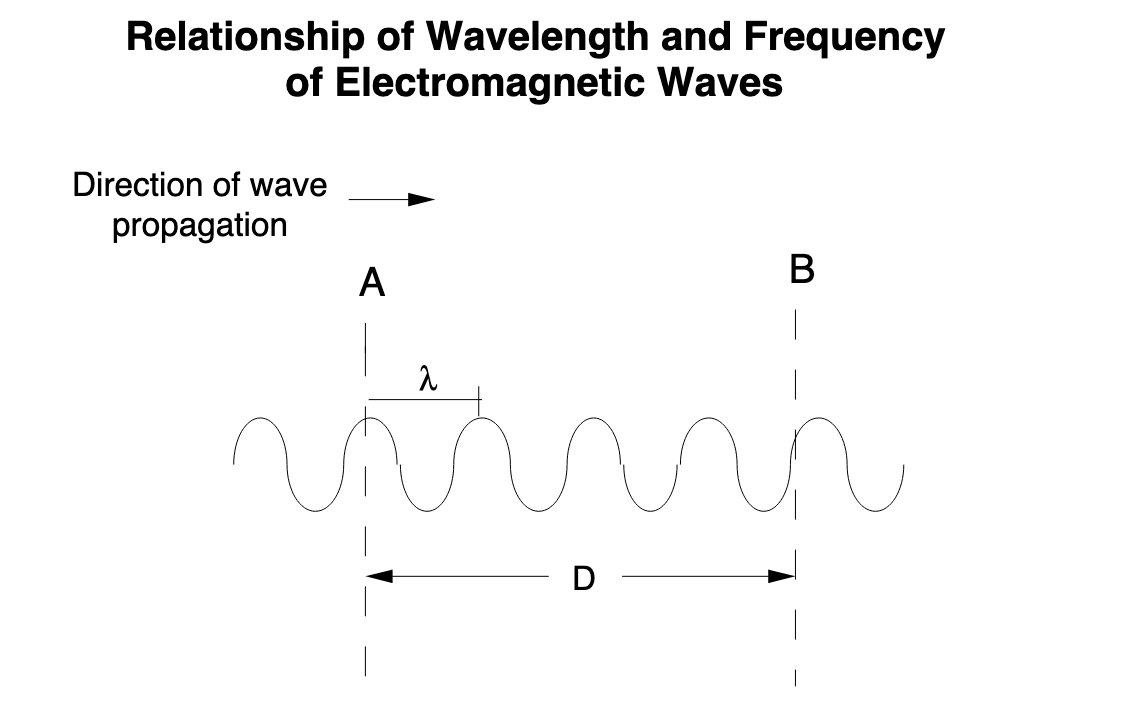
\includegraphics[width=15cm]{em wave relation.png}
    \caption{\centering \footnotesize{Relationship of Wavelength and Frequency of Electromagnetic Waves \protect\cite{NASAemradio}}}
    \label{fig:emrelation}
\end{figure}

\subsubsection{The Oscilloscope} \label{sec:1.2.1}

Oscilloscopes are device that display voltage as waves, typically sine waves, in order to visualise the variation of voltage over time
\cite{flukeoscillo,keyoscillo}.
The oscilloscope is an important device that will be used to find the resonant frequency of the LCR circuit being observed in the experiment.

\begin{figure}[H]
    \centering
    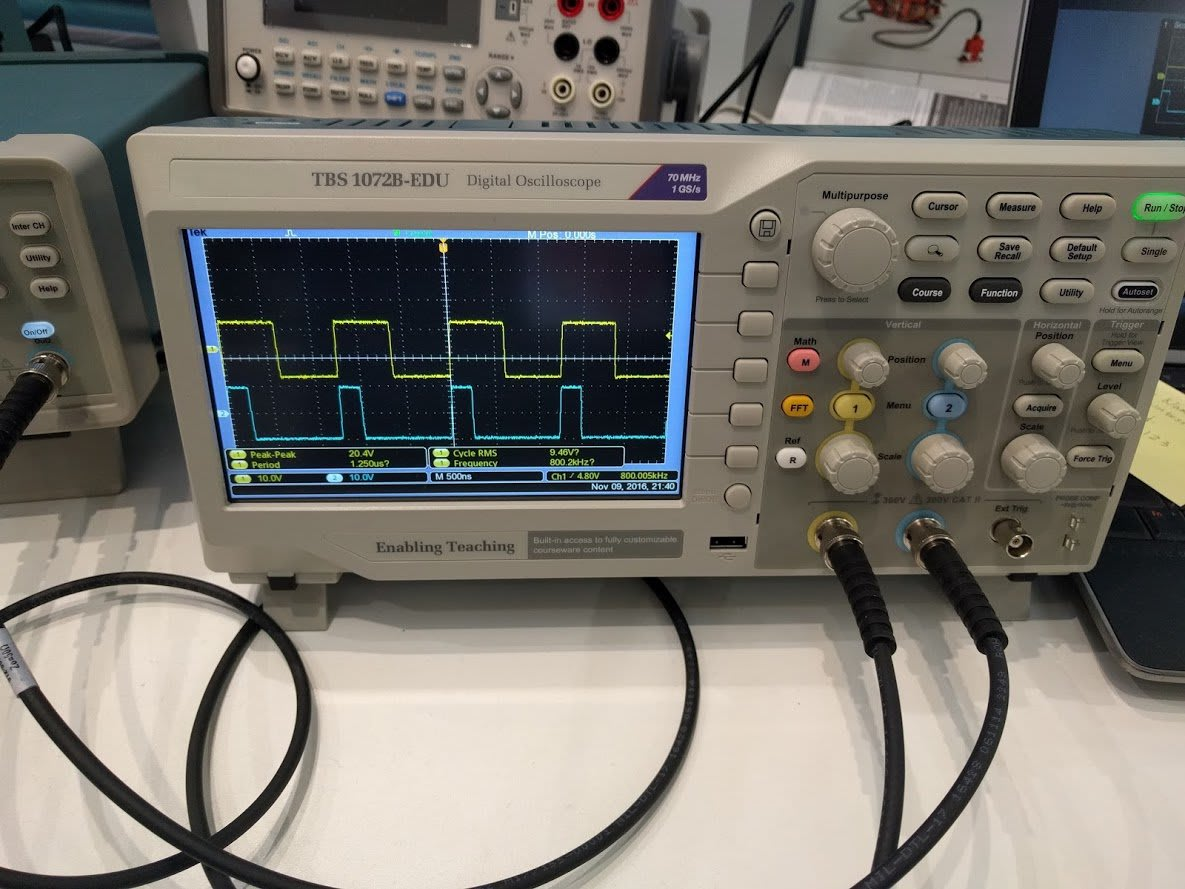
\includegraphics[width=10cm]{oscillo.jpg}
    \caption{\centering \footnotesize{Oscilloscope With 2 Channels \protect\cite{oscillopic}}}
\end{figure}

\subsubsection{Electrical Resonance} \label{sec:1.2.2}

Resonance in electrical circuits takes place at a specific, constant frequency at which the reactance and impedance cancel themselves out
\cite{geekresonance}.
The net reactance, in turn, is zero, so the current flow and voltage amplitude are increased
\cite{geekresonance}.

To get electrical resonance in a circuit the resonant frequency ($f_0$), at which the circuit is in resonance, must be found
\cite{geekresonance,eeresonance}.
Resonance, as a property of a wave, excites the particles of the same frequency. This is true even in electrical circuits.
When there net reactance is zero, the impedance in the circuit becomes entirely resistive so there is no counteraction to the flow of the current.
This constant resonance and increase in flow of current can lead to the circuit components overheating and breaking
\cite{geekresonance}.

Electical resonance will be mathematically expanded on in §\ref{sec:1.3}, The Mathematics.

\subsection{The Mathematics}\label{sec:1.3}

The reactance of the inductor $X_L$ is given by $\omega L$ where $\omega = 2 \pi f$, the angular frequency
\cite{UCDlcr,isaacimpedance}.
The reactance of the capacitor $X_C$ is given by $- \dfrac{1}{\omega C}$ with $\omega$ once again as the angular frequency
\cite{UCDlcr,isaacimpedance}.
Therefore, by understanding the total impedance formula is $\sqrt{R^2 + X^2}$
\cite{isaacimpedance},
we can then substitute X in for our two reactance values to get the impedance, Z:

\begin{gather} \label{eq:1}
    Z = \sqrt{R^2 + (X_L - X_C)^2}
\end{gather}

The current amplitude is given by $I = \dfrac{V}{Z}$, Ohm's Law, but for AC circuits extra considerations must be taken.
The AC equivalent to Ohm's Law occurs when $X_L = X_C$, where Z is then minimsed and thus the circuit will be in resonance (as discussed in §\ref{sec:1.2})
\cite{UCDlcr}.

The time domain and frequency domain are two representations of the LCR circuit, as show below in figure \ref{fig:timefreq}.

\begin{figure} [H]
    \centering
    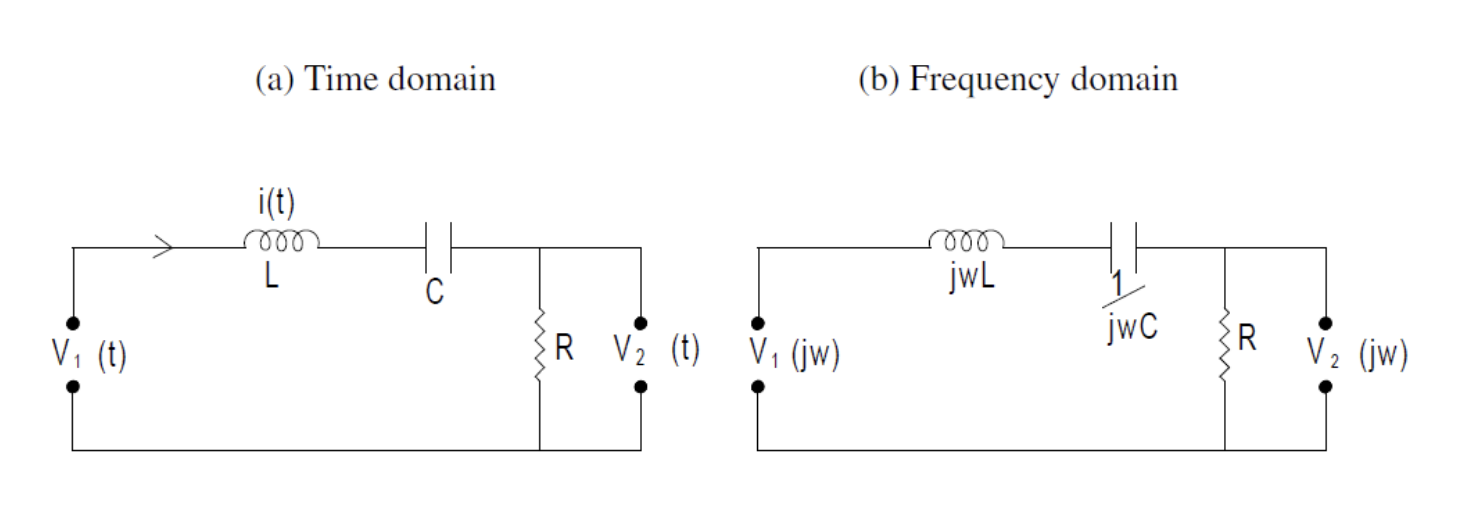
\includegraphics[width=\textwidth]{time and freq domains.png}
    \caption{\centering \footnotesize{Time and Frequency Domains of the Series LCR Circuit \protect\cite{UCDlcr}}}
    \label{fig:timefreq}
\end{figure}

With the appropriate equations below the mathematical representation becomes clearer
\cite{UCDlcr}.

Equation \ref{eq:2} represents Kirchoff's Voltage Law for series LCR circuits in the time domain, and equation \ref{eq:3} is the second-order differential equation
for the voltage that represents the time-varying response of the circuit (time domain).
Equation \ref{eq:4} is the phasor representation of the circuit in the frequency domain that takes into account the impedances from the capacitor and inductor,
as discussed in §\ref{sec:1.1.2}, the reactances. Equation \ref{eq:5} expresses the output voltage across the resistor in the frequency domain, and how the input voltage is
consequently transferred through the circuit.

\newpage
\hspace{2ex}
\begin{minipage}{0.45\textwidth}
    \begin{gather}
        v_1=L\frac{di}{dt}+\frac1C\int idt+R_1\label{eq:2}
    \end{gather}
    \vspace{-1.5em}
    \begin{gather}
        \frac{d^2v_2}{dt^2} + \frac{R dv_2}{L dt} + \frac{1}{LC} v_2 = \frac{dv_1}{dt} \cdot \frac{R}{L}\label{eq:3}
    \end{gather}
\end{minipage}
\hspace{-1.5ex}
\begin{minipage}{0.45\textwidth}
    \begin{gather}
        V_1 = j \omega L I + \frac{I}{j \omega C} + RI\label{eq:4}
    \end{gather}
    \vspace{-1.5em}
    \begin{gather}\label{eq:5}
        V_2 = IR = \frac{R}{j \omega L + \frac{1}{j \omega C} + R} V_1
    \end{gather}
\end{minipage}

\vspace{0.25cm}

\textit{Equations \ref{eq:2} and \ref{eq:3} representations of time domain. Equations \ref{eq:4} and \ref{eq:5} representations of frequency domain.} \cite{UCDlcr}

The use of complex (j) phasors in the frequency domain allows for the simplification of this above analysis by entirely removing
the need for the integro-differential equations that are in the time domain. $H(j \omega)$ is defined at the sinusoidal response function, 
the ratio of the output to the input phasor in the frequency, equation \ref{eq:6}:

\begin{gather} \label{eq:6}
    H (j \omega) = \frac{V_2}{V_1} = \frac{j \omega C R}{1 - \omega^2 L C + j \omega C R}
\end{gather}

Theoretical analysis shows that for the input signals $v_1(t) = Acos( \omega t)$ and $v_2(t) = Bcos(\omega t + \phi)$ then the gain (\ref{eq:7}) and phase shift (\ref{eq:8}) can be defined as, respectively:

\begin{gather} \label{eq:7}
    Gain \equiv \frac{B}{A} = \lvert H \rvert \: \omega CR \: \left[ (1 - \omega^2 LC)^2 + (\omega CR)^2 \right] ^ {- \frac{1}{2}}
\end{gather}

\begin{gather} \label{eq:8}
    Phase \equiv \phi = \angle H = 90 ^{\circ} - \tan^{-1} \left[ \dfrac{\omega CR}{(1 - \omega^2 LC)} \right]
\end{gather}

The behaviour of the circuit can be visualised through Bode plots, figure \ref{fig:bode}, so thus the magnitude and angle of $H(j \omega)$ determine the voltage gain and phase shift 
of a sine wave through the circuit for any measured frequency. So, $H (j \omega)$ is then considered a fundamental circuit descriptor for linear circuits \cite{UCDlcr}.

\begin{figure}[H]
    \centering
    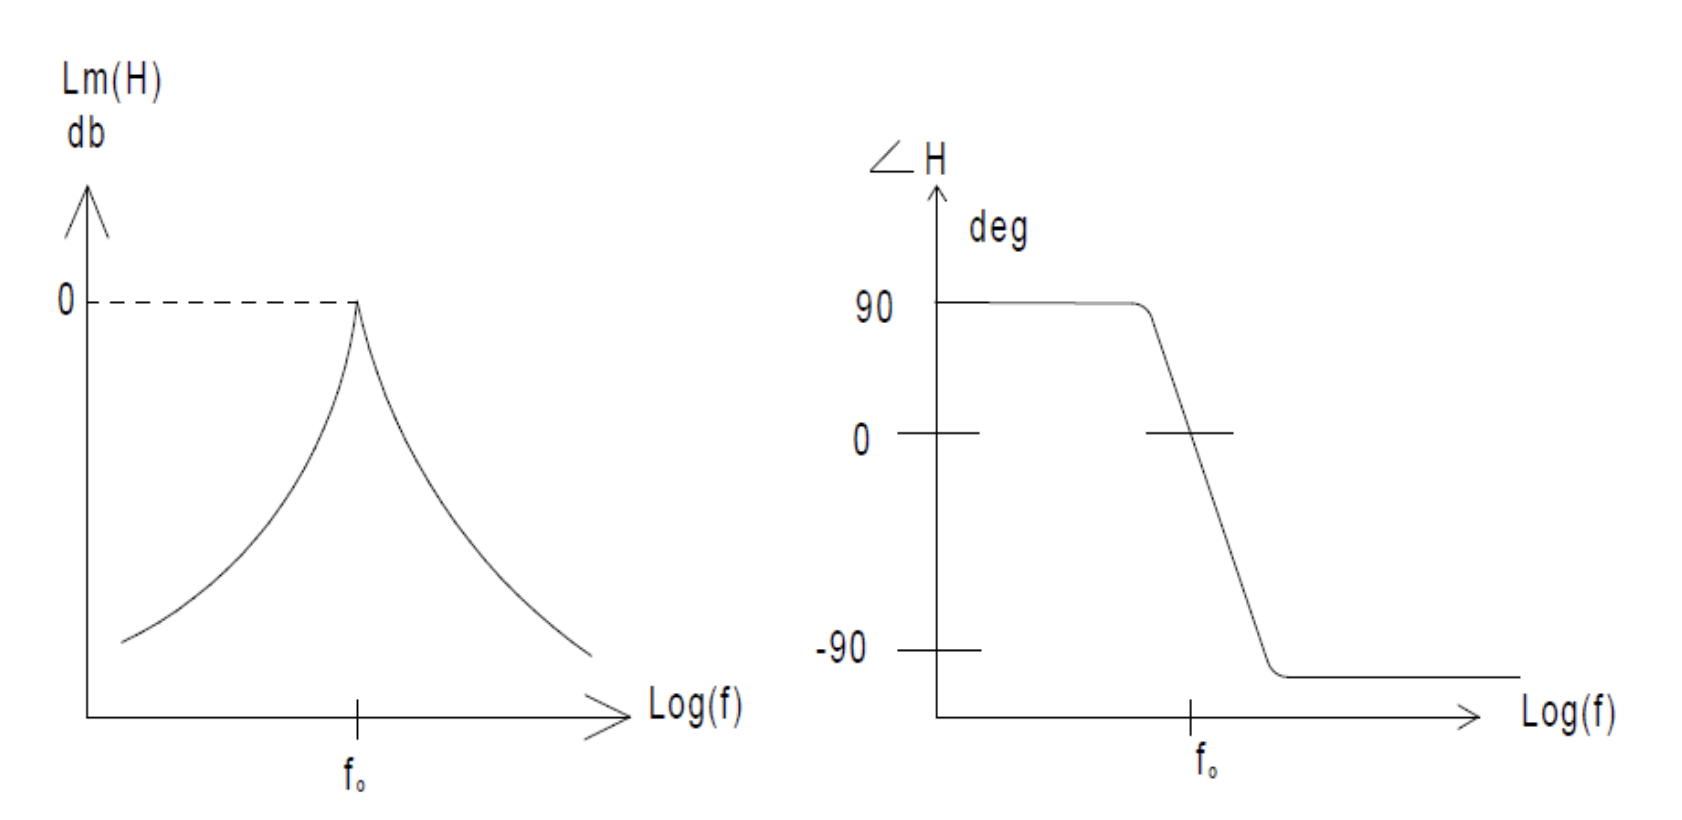
\includegraphics[width=15cm]{BODE plot.png}
    \caption{\centering \footnotesize{Typical Bode Plot Representations for the Series LCR Circuit (\textit{Magnitude: Left, Angle of $H(j \omega)$: Right}) \protect\cite{UCDlcr}}}
    \label{fig:bode}
\end{figure}

The magnitude, $Lm(H) = 20 \log_{10} (\lvert H \rvert)$, given in decibels (dB), and the angle of H, $\angle H$ are shown as functions of the logatrithm of the frequency, $\log (f)$,
which is what characterises the Bode plot for the system.
The magnitude plot shows the gain change across varying frequencies and the phase plot shows the phase shift of the circuit for varying frequencies.
The resonant frequency, $f_0$, is clearly labelled on the x-axis ($\log (f)$) for each plot, which is determined experimentally for the series LCR circuit and then 
compared to the theoretical predictions \cite{UCDlcr}.

For the LCR, the gain and phase (response) curves depend greatly on the values of L, C, and R. From equation \ref{eq:7} it can be found that
the gain reaches 0 dB, a maximum of unity, when $1 - \omega^2 LC = 0$. This observation can be used to derive the resonant frequency, $\omega_0$ or $f_0$ \cite{UCDlcr}:

\begin{gather} \label{eq:9}
    \omega_0 = \frac{1}{\sqrt{LC}} \qquad or \qquad f_0 = \frac{1}{2 \pi \sqrt{LC}}
\end{gather}

Additionally, from equation \ref{eq:8}, the phase shift ($\phi$) is seen to vary between the input and output signals with frequency such that:

\begin{itemize}
    \item At low frequencies ($\ll f_0$), the circuit has a $90^{\circ}$ phase \textbf{lead}.
    \item At high frequency ($\gg f_0$), the circuit has a $90^{\circ}$ phase \textbf{lag}.
    \item At the resonant frequency ($f_0$), the circuit phase shift passes through the $0^{\circ}$ value.
\end{itemize}

These are the typical plot behaviours illustrated in figure \ref{fig:bode} \cite{UCDlcr}.

The "sharpness" of the resonance is indicated by the narrowness of the peak in the $Lm(H)$ (gain) curve and the steepness of the phase transition through the resonant frequency.
This "sharpness" is quantified by the Q-factor, the wuality factor \cite{UCDlcr}:

\begin{gather}
    Q \; \equiv \; \frac{1}{R} \: \sqrt{\frac{L}{C}} \; = \; \frac{\omega_0 L}{R} \; = \; \frac{1}{\omega_0 RC}
\end{gather}

Greater selectivity and sharpness are a result of a higher Q-factor, shown in figure \ref{fig:bode theory}. The relationship between the gain (dB) and the phase angle ($\angle H$) is
clearly demonstrated in this graph across a range of frequencies.

\begin{figure} [H]
    \centering
    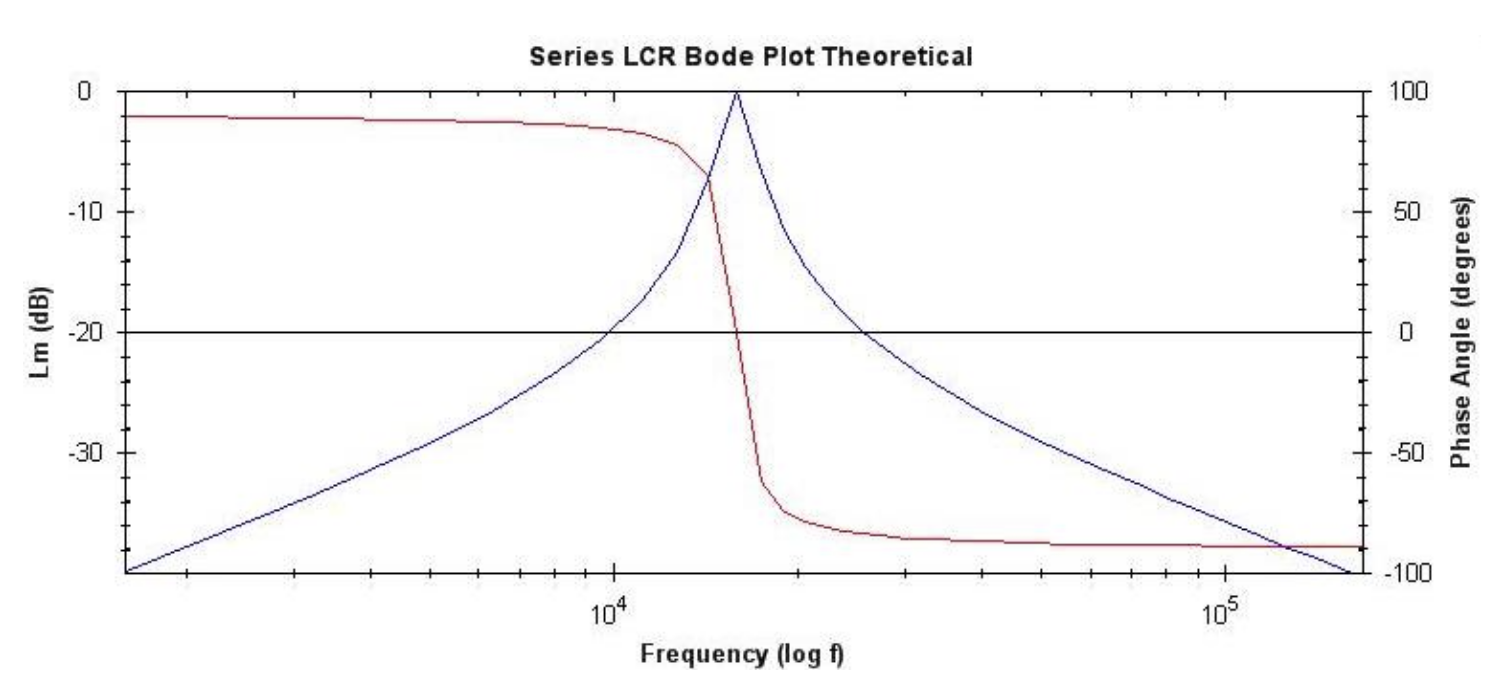
\includegraphics[width=15cm]{bode theory.png}
    \caption{\centering \footnotesize{Example of the Computer Printout for Given Values of L, C, R, and Q. The Log of the Frequency is Plotted Against the Phase Angle ($\angle H$) and the Magnitude ($Lm(H)$) \protect\cite{UCDlcr}}}
    \label{fig:bode theory}
\end{figure}

For a higher Q-factor (Q $> 10$), the selectivity for frequencies close to $f_0$ is high, which makes these circuits ideal for tuning applications, such as radios receivers, 
to isolate different transmission frequencies. These types of circuits are often referred to as a tuned circuit \cite{UCDlcr}.

For this section, the circuit is used in a similar way to a radio to tune into a specific input frequency by adjusting the resonant frequency ($f_0$).
The resonant frequency for the LCR circuit is given by \cite{UCDlcr}, similarly to equation \ref{eq:9}:

\begin{gather} \label{eq:10}
    f_0 = \frac{1}{2 \pi \sqrt{L_0C}}
\end{gather}

in which $L_0$ is the fixed inductance of the inductor, measured ealier. By varying the capacitance ($C$) the resonant frequency ($f_0$) can be varied and adjusted as well such that \cite{UCDlcr}:

\begin{gather}
    f_0 \propto \frac{1}{\sqrt{C}}
\end{gather}

This shows that decreasing the capacitance will increase the resonant frequency in an inverse square-root relationship. 
The inverse (increasing capactitance will decrease the resonant \allowbreak frequency) is also true.

It has been previously observed that the maximum gain occurs when the input frequency mathces the resonant frequency of the circuit \cite{UCDlcr}. 
Conversly, at a fixed input frequency, the input signal will be amplified to its greatest extent when the LCR circuit is tuned (by varying the capacitance $C$) to match and resonate at that input frequency.

\section{Methodology}

This experiment is composed of three sections, each with their own set of instructions:

\begin{itemize}
    \item The theoretical predictions for the LCR circuit method using plotting software, §\ref{sec:2.1}.
    \item Measurements for the Bode plot, §\ref{sec:2.2}.
    \item Measurement of the circuit response curves, §\ref{sec:2.3}.
\end{itemize}

The setup of the apparatus for the two experimental sections of this Methodology is shown in figure \ref{fig:setup}.

\begin{figure}[H]
    \centering
    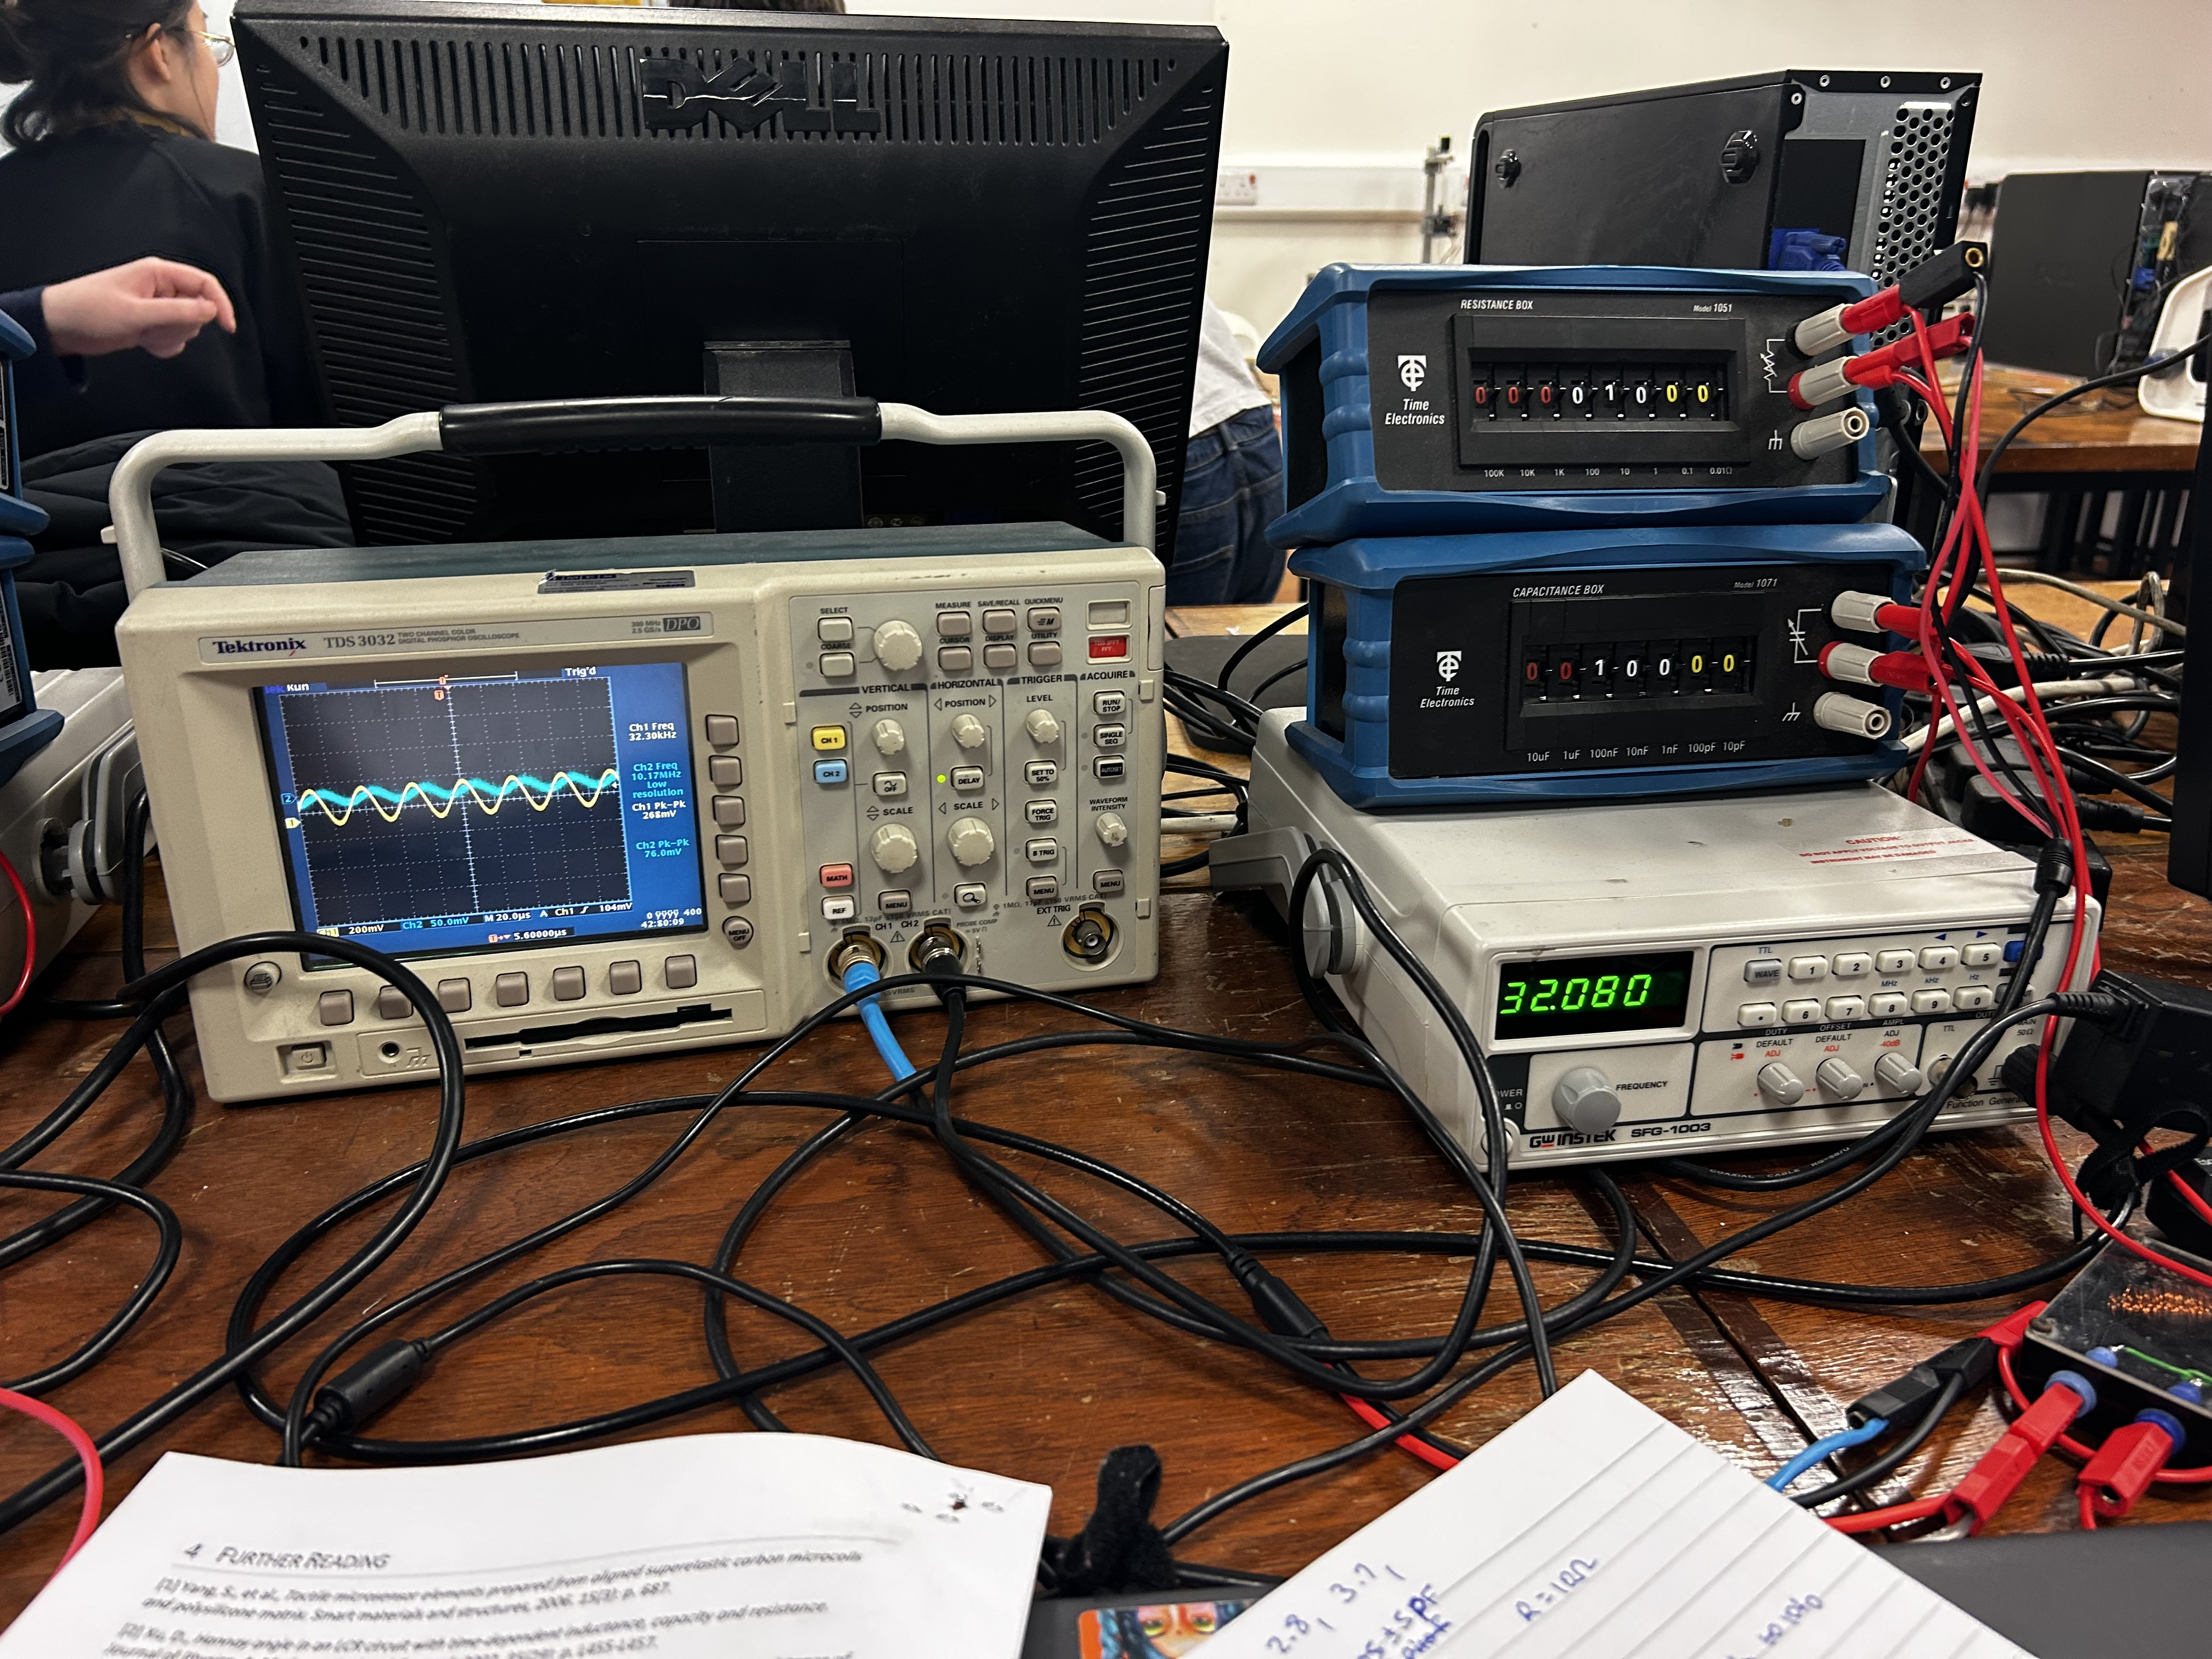
\includegraphics[width=15cm]{own exp equip.jpeg}
    \caption{\centering \footnotesize{Apparatus setup for the experimental sections.}}
    \label{fig:setup}
\end{figure}

\subsection{Theoretical Predictions for the LCR Circuit Method} \label{sec:2.1}

The "LCR Plot" program shown in figure \ref{fig:software} is opened and the values for \textbf{L}, \textbf{C}, and \textbf{R} can be set to $L=1$ mH and $C=0.1 \: \mu$F, leaving $R$ open and available
for varying values to see its effects on the plot and Q-factor.

This program calculates the resonance frequency $f_0$ and the Q-factor, plotting the predicted behaviour of the frequency response and the phase angle.
The effect of the varying \textbf{R} values on the Q-factor for a given capacitance, \textbf{C}, can be seen in figures 

The apparatus in figure \ref{fig:setup} is then assembled with \textbf{C} set to $0.1 \: \mu$F, as was done with the theory plot, and wiht \textbf{R} set to $10 \Omega$.
By observing the oscilloscope's (\textit{right}) sinewave outputs in channel 1, $\nu_1$, kept constant, and the varying amplitude via frequency changes in channel 2, $\nu_2$, the resonant frequency $f_0$
can then be found by visually comparing the sinewaves until the phase shift is close to zero. With this value of $f_0$ \textbf{L} can be calculated using equation \ref{eq:9}.

\begin{figure}[H]
    \centering
    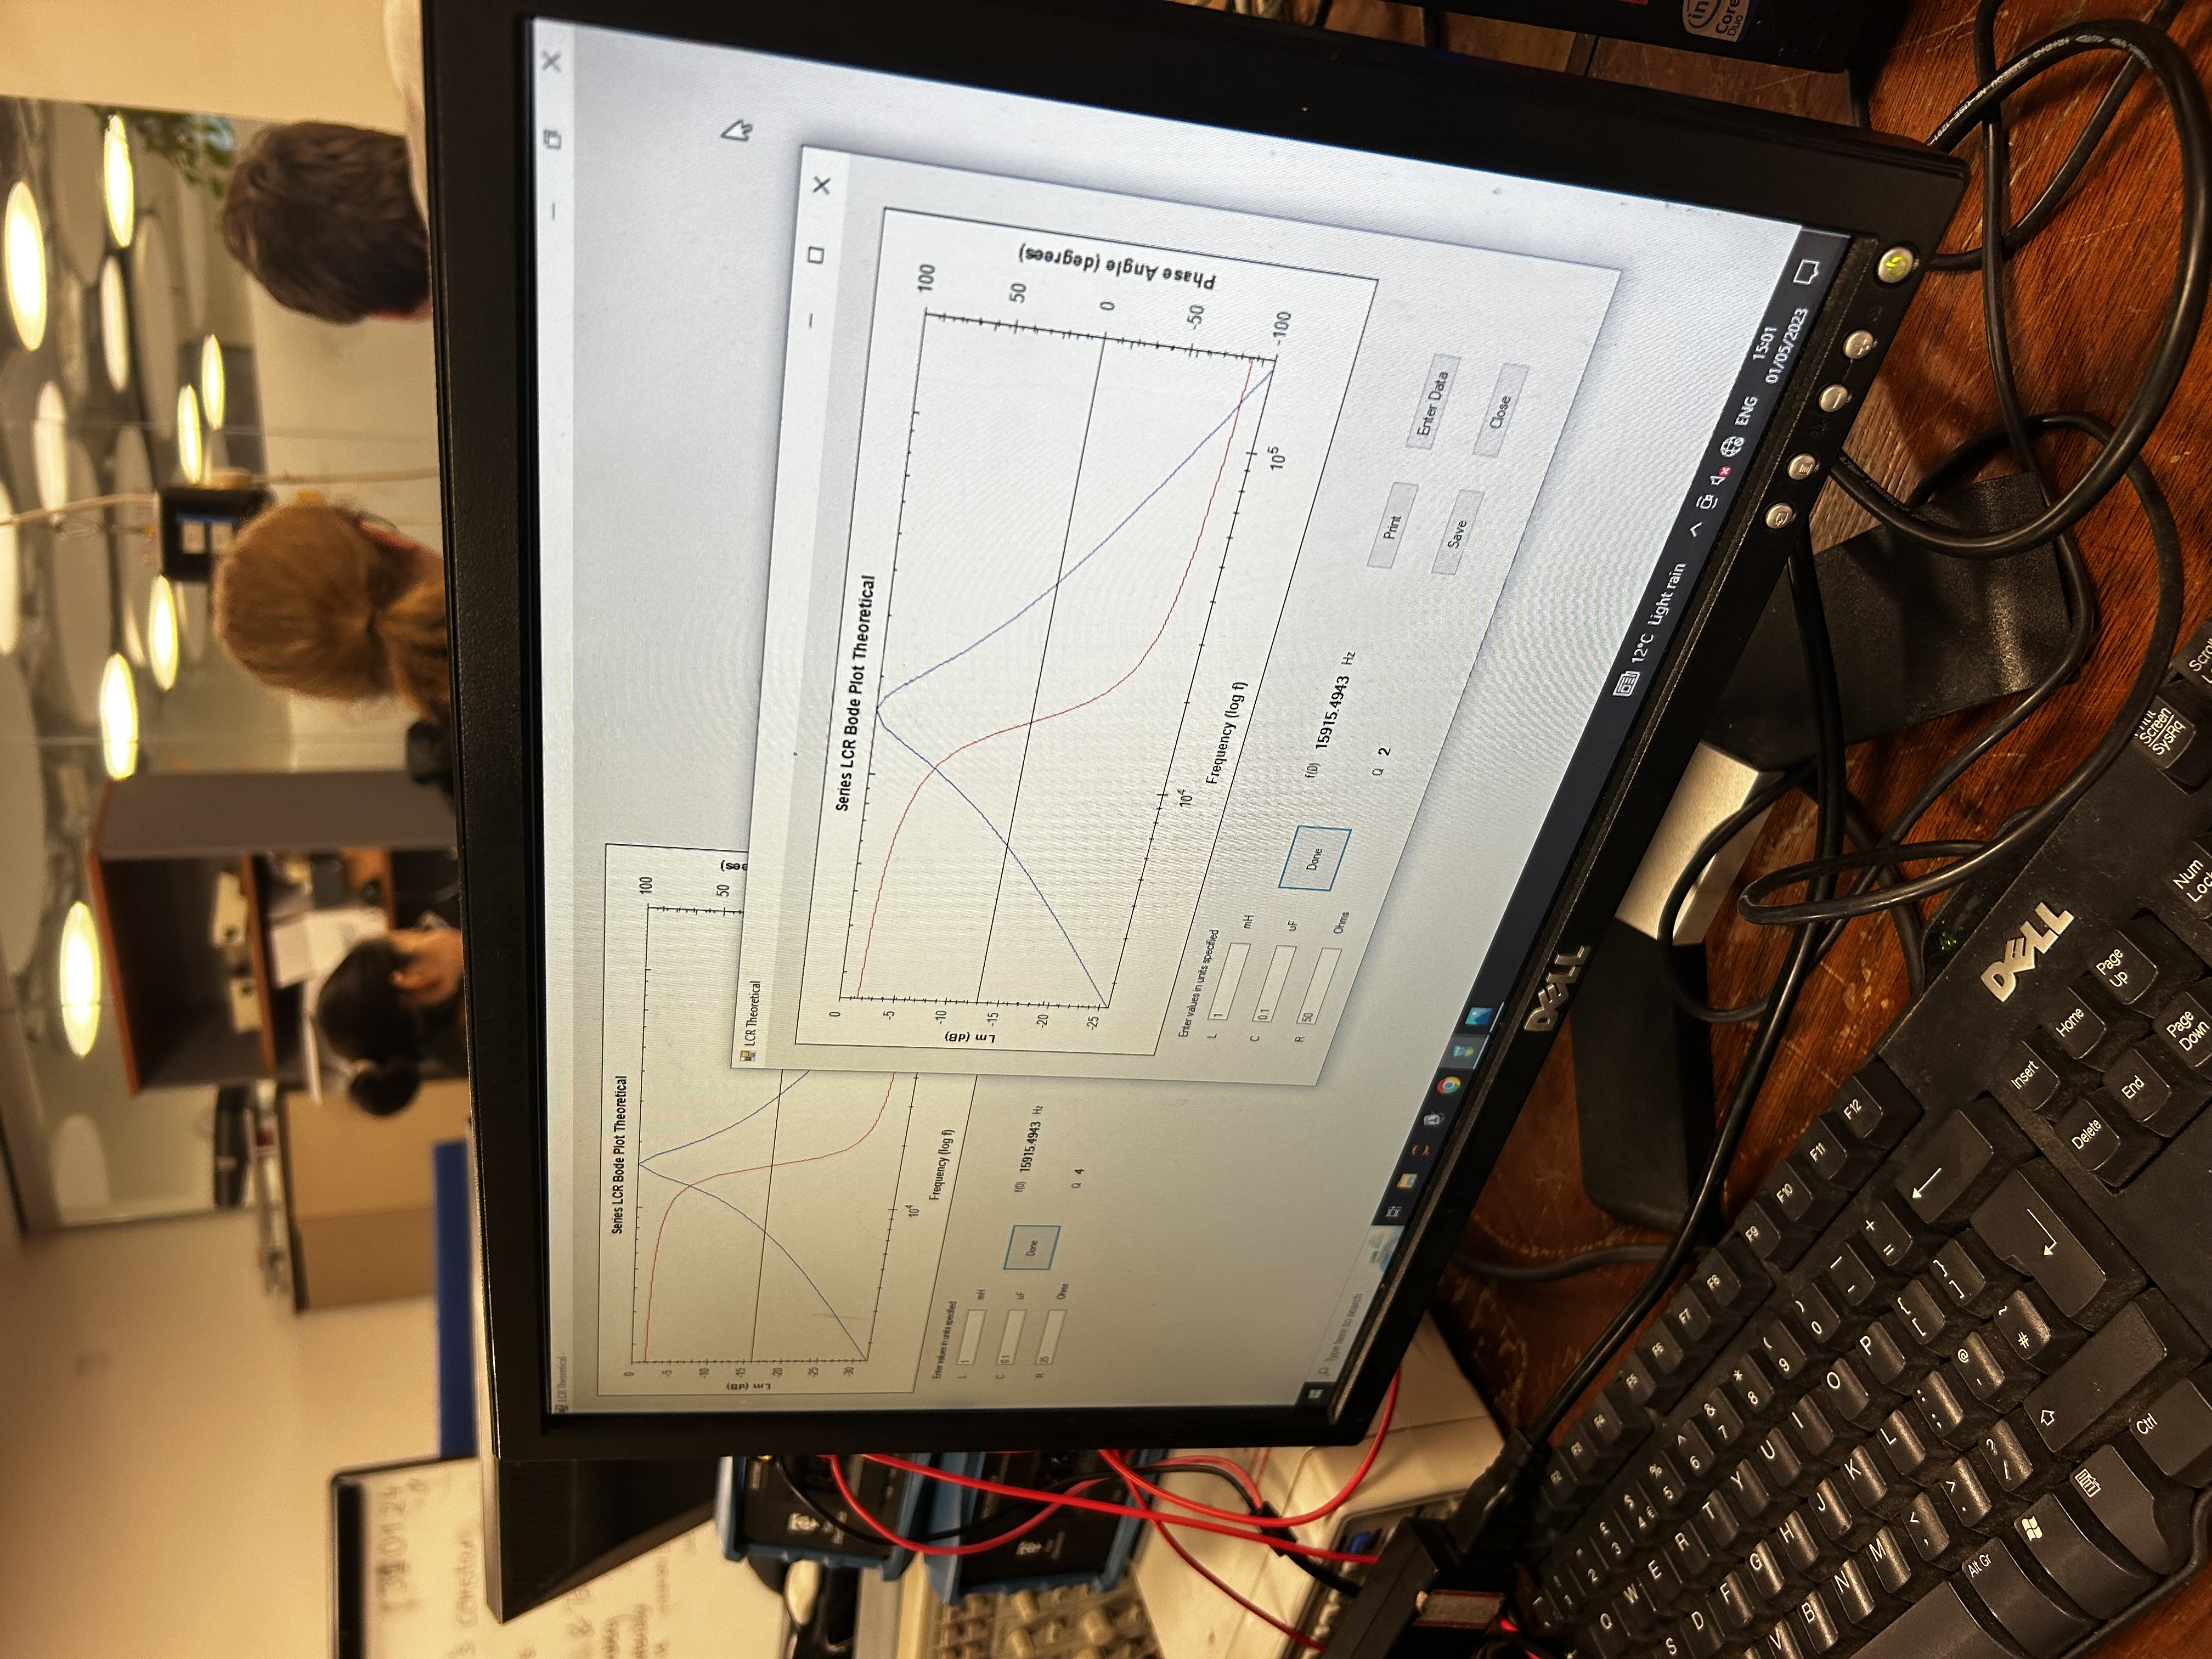
\includegraphics[width=15cm, angle=270]{own theo exp.jpeg}
    \caption{\centering \footnotesize{Theoretical software for the prediction of the LCR circuit.}}
    \label{fig:software}
\end{figure}

\subsection{Measurements for the Bode Plot Method} \label{sec:2.2}

The behaviour of the LCR circuit is studied with varying input frequency while \textbf{L}, \textbf{C}, and \textbf{R} remain fixed.
Measurements for this behaviour are taken in logatrithmic increments over two decades are selected (\textit{ie,} $0.1f_0$ \textit{to} $10f_0$) and values for the input and output peak-to-peak
voltages are noted.
The phase shift is achieved by measuring the time difference, $\Delta T$, between the peaks and noting whether the phase shift is \textbf{lag} or \textbf{lead}.
More readings should be taken closer to resonance, in which the set frequencies ideally provide evenly distributed data points to either side of the resonant frequency
on a log-axis scale.

The gain (in dB) can be computed using the formula:

\begin{gather} \label{eq:13}
    (Lm(\lvert H \rvert))(dB) \: = \: 20 \log_{10} \frac{\nu_2}{\nu_1}
\end{gather}

The phase shift (in degrees) can be determined by the formula:

\begin{gather} \label{eq:14}
    \angle H (^{\circ}) \: = \: 360 \: \times \: f \: \times \: \Delta T
\end{gather}

\subsection{Measurement of the Circuit Response Curves Method} \label{sec:2.3}

The circuit's response to varying capacitance, \textbf{C}, is investigated by setting the resistance to $R= 10 \Omega$ and the resonant frequency to what was measured in §\ref{sec:2.1} and keeping these values constant.
The values of C are varied around the resonance with as fine of a scale as possible that allows a symmetrical and smooth graph to be produced. For each C value taken, the corresponding output frequecy is recorded from the oscilloscope.
A graph like what is illustrated in figure \ref{fig:lcrresponsecurve} below should be the aim of what is produced with these measurements.

\begin{figure}[H]
    \centering
    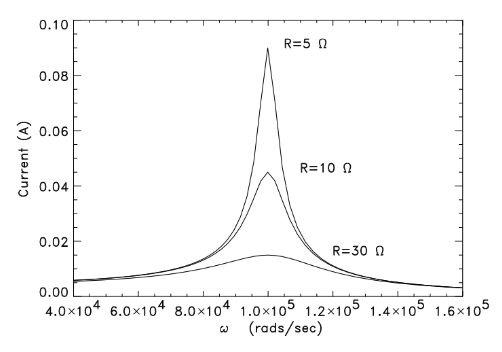
\includegraphics[width=15cm]{graph LCR goof.png}
    \caption{\centering Theoretical response curves for the LCR series circuit assuming an input voltage amplitude of 0.45V. \protect\cite{UCDlcr}}
    \label{fig:lcrresponsecurve}
\end{figure}

The above steps are repeated for a constant $R = 30 \Omega$ and, if time were to permit, would have also been recreated for a constant $R = 5 \Omega$. The input frequency is kept constant throughout.

\section{Results and Calculations}

\subsection{Theoretical Predictions for the Bode Plot} \label{sec:3.1}

\textit{The results for this section were obtained by following the method procedure in from §\ref{sec:2.1}.}

The figures for the theoretical Bode plots simulated for specificied values of \textbf{R} can be found in the Appendix, §\ref{sec:A.1.1}.

\begin{itemize}
    \item For $R = 5 \Omega$, figure \ref{fig:R5} shows the theoretical Bode plot.
    \item For $R = 10 \Omega$, figure \ref{fig:R10} shows the theoretical Bode plot.
    \item For $R = 20 \Omega$, figure \ref{fig:R20} shows the theoretical Bode plot.
    \item For $R = 30 \Omega$, figure \ref{fig:R30} shows the theoretical Bode plot.
    \item For $R = 40 \Omega$, figure \ref{fig:R40} shows the theoretical Bode plot.
    \item For $R = 50 \Omega$, figure \ref{fig:R50} shows the theoretical Bode plot.
\end{itemize}

\vspace{0.25cm}

After simulating these plots, the resonant frequency for the LCR circuit was calculated and found. At the resistance of $R = 10 \Omega$ and capacitance of $C = 0.1 \mu$F, as was
specified in §\ref{sec:2.1}, the resonant frequency was discovered to approximately be:

\begin{gather} \label{eq:15}
    f_0 \: = \: 16040 \: \text{Hz} \: \pm \: 0.5 \: \text{Hz}
\end{gather}

With the use of this found resonant frequency value, the inductance, \textbf{L}, was calculated via a manipulation of equation \ref{eq:9}:

\begin{gather} \label{eq:16}
    f_0 = \frac{1}{2 \pi \sqrt{LC}} \: \implies \: \left( \frac{1}{2 \pi f_0} \right)^2 = LC \: \implies \:
    L = \frac{1}{4 \pi^2 f_0^2 C}
\end{gather}

With the substitution for the values of $f_0 = 16040$Hz and $C = 0.1 \mu$F:

\begin{gather} \label{eq:17}
    L \: = \: \frac{1}{4 \pi^2 (16040)^2 (0.1 \times 10^{-6})} \: = \: 9.845 \times 10^{-4} \: \text{H} \: \pm \: 
\end{gather}

Where the unit for inductance is the \textit{Henry (H)}.

\subsection{Measurements for the Bode Plot} \label{sec:3.2}

\renewcommand{\arraystretch}{1.3}

\begin{table}[H] 

    \centering
    \resizebox{\textwidth}{!}{

        \begin{tabular}{|c|c|c|c|c|c|c|c|}
        \hline
        Log $f_0$ & \begin{tabular}[c]{@{}c@{}}Frequency\\ (Hz)\end{tabular} & \begin{tabular}[c]{@{}c@{}}Ch1, $\nu_1$\\ (V)\end{tabular} & \begin{tabular}[c]{@{}c@{}}Ch1, $\Delta \nu_1$\\ (V)\end{tabular} & \begin{tabular}[c]{@{}c@{}}Ch2, $\nu_2$\\ (V)\end{tabular} & \begin{tabular}[c]{@{}c@{}}Ch2, $\Delta \nu_2$\\ (V)\end{tabular} & \begin{tabular}[c]{@{}c@{}}$\Delta T$\\ (s) $\times 10^{-6}$\end{tabular} & \begin{tabular}[c]{@{}c@{}}$\Delta (\Delta T)$\\ (s) $\times 10^{-6}$\end{tabular} \\ \hline
        $0.1 f_0$ & $1 \: 604$                                               & 0.28                                                       & 0.004                                                             & 0.043                                                      & 0.01125                                                           & 240                                                                       & 80                                                                                 \\ \hline
        $0.3 f_0$ & $4 \: 812$                                               & 0.28                                                       & 0.006                                                             & 0.06                                                       & 0.019                                                             & 50                                                                        & 5                                                                                  \\ \hline
        $0.5 f_0$ & $8 \: 020$                                               & 0.272                                                      & 0.004                                                             & 0.0732                                                     & 0.038                                                             & 32                                                                        & 8                                                                                  \\ \hline
        $0.8 f_0$ & $12 \: 832$                                              & 0.2                                                        & 0.004                                                             & 0.89                                                       & 0.0145                                                            & 16                                                                        & 2                                                                                  \\ \hline
        $f_0$     & $16 \: 040$                                              & 0.084                                                      & 0.006                                                             & 0.84                                                       & 0.006                                                             & 0                                                                         & 4                                                                                  \\ \hline
        $3 f_0$   & $48 \: 120$                                              & 0.284                                                      & 0.004                                                             & 0.0551                                                     & 0.0156                                                            & 6                                                                         & 1                                                                                  \\ \hline
        $5 f_0$   & $80 \: 200$                                              & 0.284                                                      & 0.006                                                             & 0.062                                                      & 0.0076                                                            & 3.2                                                                       & 2                                                                                  \\ \hline
        $8 f_0$   & $128 \: 320$                                             & 0.284                                                      & 0.006                                                             & 0.055                                                      & 0.012                                                             & 2                                                                         & 1                                                                                  \\ \hline
        $10 f_0$  & $160 \: 400$                                             & 0.27                                                       & 0.004                                                             & 0.03                                                       & 0.01                                                              & 1.6                                                                       & 0.2                                                                                \\ \hline
        \end{tabular}

    }

    \caption{\centering Table of the data collected to generate a Bode plot.}
    \label{tab:1}

\end{table}

\subsection{Measurement of the Circuit Response Curves} \label{sec:3.3}



\section{Conclusion}



\section{Applications of Electrical Resonance}




\newpage


%%%%%%%%%%%%%%%%%%%%%%%%%%%%%%%%%%%

\bibliographystyle{IEEEtran}
\bibliography{References}


\newpage

\section*{Appendix} \label{sec:A}
\addcontentsline{toc}{section}{Appendix}

\subsection*{Raw Data} \label{sec:A.1}
\addcontentsline{toc}{subsection}{Raw Data} 

\subsubsection*{Graphs for the Simulated Theoretical Predictions for the Bode Plot} \label{sec:A.1.1}

\vspace{1cm}

\begin{minipage}{0.45\textwidth}
    \captionsetup{hypcap=false}
    \centering
    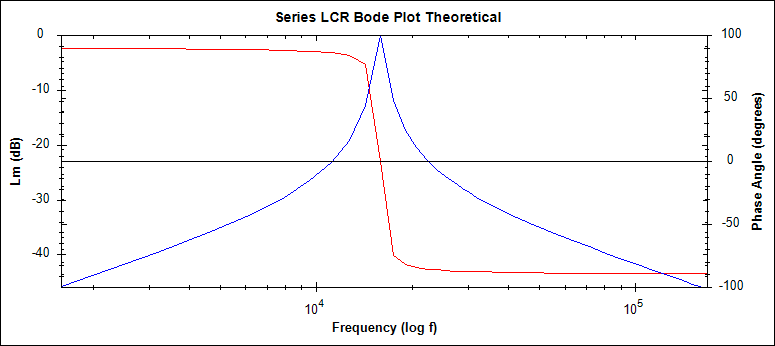
\includegraphics[width=.9\linewidth]{plot R5.png}
    \captionof{figure}{Theoretical Bode Plot, $R= 5 \Omega$}
    \label{fig:R5}

    \vspace{1.5em}
    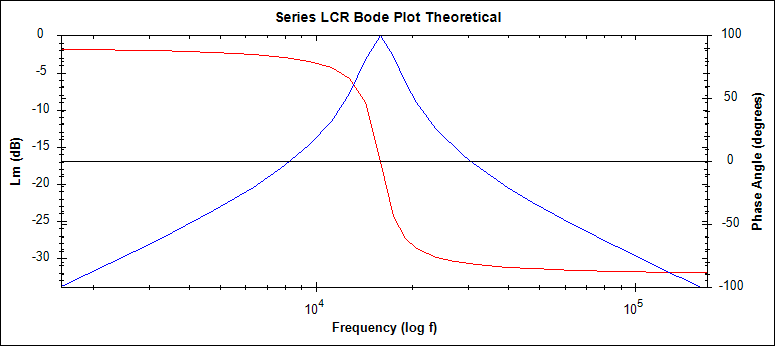
\includegraphics[width=.9\linewidth]{plot R20.png}
    \captionof{figure}{Theoretical Bode Plot, $R = 20 \Omega$}
    \label{fig:R20}

    \vspace{1.5em}
    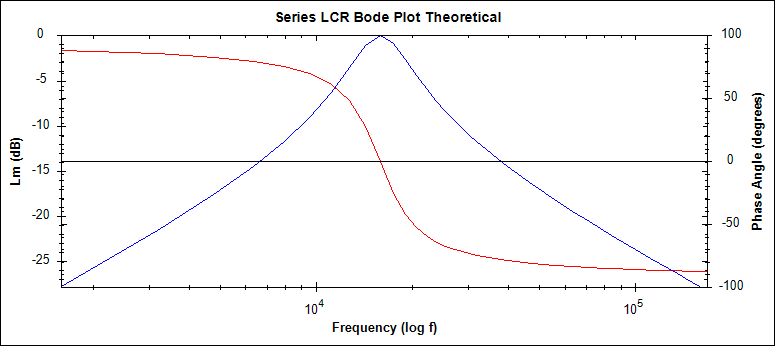
\includegraphics[width=.9\linewidth]{plot R40.png}
    \captionof{figure}{Theoretical Bode Plot, $R = 40 \Omega$}
    \label{fig:R40}
\end{minipage}
\hfill
\begin{minipage}{0.45\textwidth}
    \captionsetup{hypcap=false}
    \centering
    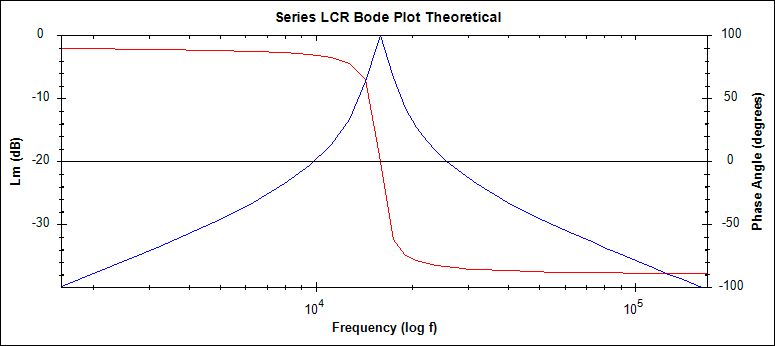
\includegraphics[width=.9\linewidth]{plot R10.png}
    \captionof{figure}{Theoretical Bode Plot, $R= 10 \Omega$}
    \label{fig:R10}

    \vspace{1.5em}
    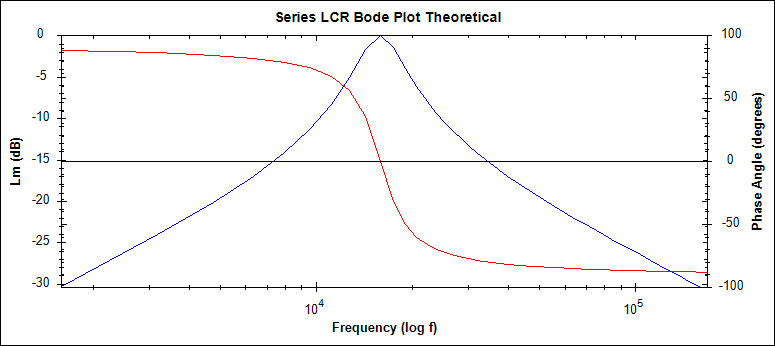
\includegraphics[width=.9\linewidth]{plot R30.png}
    \captionof{figure}{Theoretical Bode Plot, $R = 30 \Omega$}
    \label{fig:R30}

    \vspace{1.5em}
    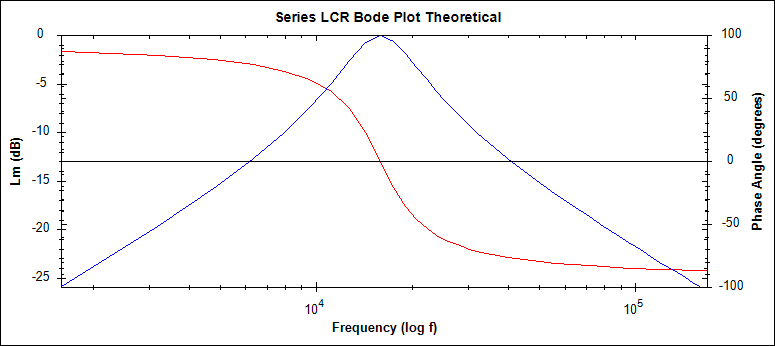
\includegraphics[width=.9\linewidth]{plot R50.png}
    \captionof{figure}{Theoretical Bode Plot, $R = 50 \Omega$}
    \label{fig:R50}
\end{minipage}%

\vspace{1cm}

\subsection*{Code}
\addcontentsline{toc}{subsection}{Code}

\listoffigures

\listoftables

\end{document}